\documentclass[11pt]{article}\usepackage[]{graphicx}\usepackage[]{color}
% maxwidth is the original width if it is less than linewidth
% otherwise use linewidth (to make sure the graphics do not exceed the margin)
\makeatletter
\def\maxwidth{ %
  \ifdim\Gin@nat@width>\linewidth
    \linewidth
  \else
    \Gin@nat@width
  \fi
}
\makeatother

\definecolor{fgcolor}{rgb}{0.345, 0.345, 0.345}
\newcommand{\hlnum}[1]{\textcolor[rgb]{0.686,0.059,0.569}{#1}}%
\newcommand{\hlstr}[1]{\textcolor[rgb]{0.192,0.494,0.8}{#1}}%
\newcommand{\hlcom}[1]{\textcolor[rgb]{0.678,0.584,0.686}{\textit{#1}}}%
\newcommand{\hlopt}[1]{\textcolor[rgb]{0,0,0}{#1}}%
\newcommand{\hlstd}[1]{\textcolor[rgb]{0.345,0.345,0.345}{#1}}%
\newcommand{\hlkwa}[1]{\textcolor[rgb]{0.161,0.373,0.58}{\textbf{#1}}}%
\newcommand{\hlkwb}[1]{\textcolor[rgb]{0.69,0.353,0.396}{#1}}%
\newcommand{\hlkwc}[1]{\textcolor[rgb]{0.333,0.667,0.333}{#1}}%
\newcommand{\hlkwd}[1]{\textcolor[rgb]{0.737,0.353,0.396}{\textbf{#1}}}%
\let\hlipl\hlkwb

\usepackage{framed}
\makeatletter
\newenvironment{kframe}{%
 \def\at@end@of@kframe{}%
 \ifinner\ifhmode%
  \def\at@end@of@kframe{\end{minipage}}%
  \begin{minipage}{\columnwidth}%
 \fi\fi%
 \def\FrameCommand##1{\hskip\@totalleftmargin \hskip-\fboxsep
 \colorbox{shadecolor}{##1}\hskip-\fboxsep
     % There is no \\@totalrightmargin, so:
     \hskip-\linewidth \hskip-\@totalleftmargin \hskip\columnwidth}%
 \MakeFramed {\advance\hsize-\width
   \@totalleftmargin\z@ \linewidth\hsize
   \@setminipage}}%
 {\par\unskip\endMakeFramed%
 \at@end@of@kframe}
\makeatother

\definecolor{shadecolor}{rgb}{.97, .97, .97}
\definecolor{messagecolor}{rgb}{0, 0, 0}
\definecolor{warningcolor}{rgb}{1, 0, 1}
\definecolor{errorcolor}{rgb}{1, 0, 0}
\newenvironment{knitrout}{}{} % an empty environment to be redefined in TeX

\usepackage{alltt}
%Required: You must have these
\usepackage{graphicx}
\usepackage{tabularx}
\usepackage{natbib}
\usepackage{array}
\usepackage{amsmath}
\usepackage{rotating}

%\usepackage[backend=bibtex]{biblatex}


\setkeys{Gin}{width=0.8\textwidth}
%\setlength{\captionmargin}{30pt}
\setlength{\abovecaptionskip}{10pt}
\setlength{\belowcaptionskip}{10pt}

 \topmargin -1.5cm 
 \oddsidemargin -0.04cm 
 \evensidemargin -0.04cm 
 \textwidth 16.59cm
 \textheight 21.94cm 
 \parskip 7.2pt 
\renewcommand{\baselinestretch}{1.6} 	
\parindent 0pt


\bibliographystyle{..//refs/styles/besjournals.bst}
\usepackage{xr-hyper}
%\usepackage{hyperref}
%\externaldocument{SUPP_FLS_flobud}

\title{Seasonal priority effects alter the competitive dynamics of temperate forest herbs }
\IfFileExists{upquote.sty}{\usepackage{upquote}}{}
\begin{document}
\maketitle


\section*{Introduction}
\noindent A core task of community ecology is explain patterns of community assembly across a diversity of ecosystems \citep{Weiher:2011aa}. A central tenet of community assembly theory is that the order of arrival of species to a community mediates inter-specific interactions and can dictate the trajectory of community structure in the long term \citep{Fukami2015}. These historical contingencies, known as priority effects, have been shown to alter the structure and function of communities, driving communities to alternate stable states \citep{Fukami2011}.\\

\noindent In many ecosystems, plant communities must re-assemble each year after a period of dormancy. In these communities, priority effects are largely the product of the rate at which dormant plants and seeds respond to their environment and resume growth or germinate when favorable conditions return \citep{Rudolf:2019aa}, rather than the the timing of the arrival of propagules, which in many cases occurs prior to the dormant season \citep{Howe:1982aa,Baskin:1988aa}.  These seasonal, or short-term priority effects (SPEs) \citep{Wainwright_2011,Young:2017aa}, may be important mediators of plant interactions, and have been invoked to explain both the invasion success and competitive dominance of some species (when strong competitors also have rapid/early germination) \citep{Gioria2018}, and inter-specific coexistence (when weaker competitors have rapid/early germination and/or priority varies over time) \citep{Towers:2020aa}.\\

\noident While this evidence suggests priority effects may be important in regulating community interactions, it is unclear to what extent these patterns are broadly generalizable. First, almost all mechanistic tests for SPEs to date have been performed using species from temperate grasslands \citep{Weidlich:2020aa}, whose germination behavior may differ substantially from taxa in other habitats \citep{Tudela-Isanta:2018aa}. Second, the evidence for SPE's comes primarly from experiments that stagger the planting time of competing species \citep{Young:2017aa,Letten:2018aa}. A recent review paper by \citet{Weidlich:2020aa} reported that of 42 out of the 43 studies they evaluated found evidence for priority effects, and 18 of those studies (42\%) included planting interval treatments of less than 1 month, approximating the time scale of SPEs. However, it is unclear if the large germination intervals (time between plantings) applied in these experiments are realistic proxies for the intervals that occur under natural conditions, where germination is primarily dictated by the environment.\\

\noindent Research suggests that the timing of germination is controlled by environmental cues---temperature (both cool stratification temperatures to break dormancy and warm incubation temperatures to stimulate germination), moisture and light availability \citep{Bewley1997,Fenner2000}. Because the seed bank of any community experiences the same environment at a given time, it is possible that the species in that community have evolved similar responses to environmental variation, which appears to be true at the global scale \citep{Rubio-de-Casas:2017aa}. In this case, the timing between species' germination events may differ, but this interval would remain constant in both favorable and unfavorable germination years (Fig. \ref{}a). If this the case, it is impossible to disentangle the contribution of germination priority and other competitive traits, which often co-vary with rapid germination \citep{Dickson2012}, to competitive dominance.\\ 

\noindent Alternatively, while competing species may evolve to share germination cues, their sensitivity ($\Delta$ germination rate$/\Delta$ cue) to these cues may differ substantially. In this scenario, inter-annual climate variation would generate inter-annual variation in the strength of SPEs (Fig. \ref{}b). These dynamics would allow researchers to quantify the contribution of the priorty effects to competition. %Additionally variation in SPEs introduce enough temporal differences in competitor's per capita competitive abilities to suggest that sufficiently environmental variation would allow them to co-exist via the storage effect \citep{}.

\noindent Assessing the role of SPE's in species interactions under more realistic germination environments and is particularly important and timely as anthropogenic climatic change is altering the germination environments of species across the globe \citep{Walck2011}.  Such sustained alterations to environmental cues have potential to disrupt SPEs, shifting balances of species' interactions, and impacting population demography, community composition and ecosystem functions.\\ 

\noindent To address this we performed a series of experiments to both quatify the the relationship between SPEs and environmental variation and how these climate driven differences in SPEs impact inter-specific competition. First, we quantified the differences in germination rate responses to temperature variation for a suite of herbaceous species found in temperate forests with full-factorial growth-chamber experiment in which we manipulated the duration of stratification and incubation temperatures. Second we planted two species from our first trial in competition and exposed them to two different levels of cold stratification which, generating variation SPEs among treatments. From this secondary case study were were able to quantify the contribution of SPE's to the competitive dynamics among these species, and used these results to parameterize a simple competional model to forcast the competitive dynamics of these species under varying cliamte conditions.

\section*{Methods}
\subsection{Quantifying relationship between SPE's and Environmental varition}
\subsubsection*{Experimental Design}
To investigate the relationship between environmental varition and germination timing, we randomly assigned seeds of 14 herbaceous plant speces to a  fully crossed set of twenty experimental treatments; 10 levels of of cold stratification duration (0,14,days at 4\degree C) , two levels of incbation temperature (25\degree C:15\degree C (day/night) warm vs 20\degree C:10\degree C (day/night) cool). To maximize the amount of germination niche diversity in our sample we chose a mix of spring-germinating species common to temperate forest edge and understory habitats including both native and exotic species with known variation in dormancy class and habitat specialization. The full list of species can be found in Fig. \ref{}.\\
\noindent  We obtained seeds of most species from plant nurseries, but for two species we, collected seeds locally afrom unmanaged habitat at the Arnold Arboretum in Boston MA Coordinates). Prior to applying experimental treatments we applied a ``float test" in which all seeds were placed in distilled water and unfilled seeds (floating) were removed from the experiment \citep{}. The remaining seeds were imbibed in distilled water for 24 hours after which we placed  20 seeds per species/ treatment combinationwere place in petri dish on a single layer of moist filter paper on top of filter sand. We replicated each treatment combination 3 times. For the cold stratification treatments, we wrapped petri dishes in aluminum foil to prevent light exposure and placed them in a growth chamber at 4\degree C. After each stratification interval, we transfered the petri dishes to their assigned incubation chamber for 25 days, moistening the germination substrate as neccisary to maintain maximum saturation of the medium with out flooding the seeds. We check for new germinates every 2 days, defining a seed as germinated when its radical or cotolyden tissue was visable.  \citep{}. We assessed the viability of any seeds that did not germinate in the 25 day incubation trial by performing a ``crush test" in which we applied pressire to the intact seed to evaluate its condition \citepP{}. We excluded any subsequent seeds deemed deemed unviable from all subsequent analyses. Due to the staggering of our stratification treatments the experiment took place between 27 August- 12 December 2018.\\

\subsubsection*{Statistical analysis}
To assess interspecific differences in the relationship between germination rate and temperature variability, we fit a Bayesian mixed-effect accelerated failture time model (AFT) with weeks of stratification and incubation temperature as fixed effects and species as a grouping factor on both the model's slopes and intercepts. Three species, \textit{Phlox cuspidata},\textit{Impatiens capensis} and \textit{Carex grisea}did not germinate well under any of our treatment so we excluded them from out model, leaving 11 species for our analysis. We chose an AFT model as it allowed for us to account for viable seeds that did not germinate during our inclubation window letting us robustly compare germination timing (t50 time to 50\% germination) even among species and treatment with different final germination percentages \citep{Soltani:2015aa}. One drawback of this approach is that these classes models assume that all viable seeds will eventually germination, an assumption which we would not expect to be true in nature. For this reason, we considered any estimate t50 values greater than 60 days to suggest that particular seed lot would not reach 50\% germination under those conditions.\\ %%woof say better.

\noindent We fit the model using the R package ``brms" \citep{Burkner2018} using a weibull distrubtion for the model's likelihood function. We ran the model on four chains with 4000 iterations and a 3000 iteration warm up for a total of 4000 posterior draws for each parameter using weakly informative priors. We assessed  model performance through ensuring $\hat{R}$s were between 1 and 1.01 and bulk and tail effective sample sizes were high.

\subsection{Two species case study}
\subsubsection*{Experimental Design}
To quatify the contribution of SPEs to inter-specific competition dynamics, we chose two species from our germination trial \textit{Cryptotaenia canadensis} and \textit{Hesperis matronalis} for competion trials. We chose these species because the germination of \textit{C. candensis} advanced strongly with increasing cold stratification, while seeds of \textit{H. matronalis} germinated rapidly under all conditions suggesting that under low stratification treatments there would be a stong priority effect between the species that would diminish as stratifaction time increased. Additionally \texit{H. matronilis},originially from Eurasia, is considered an invasive species or noxious weed in many parts of North America and so evaluating the role of SPE's in this species's comptetitive ability has potential applied benefits for the management of this species.\\

\noindent Competition trials took place under contolled condition in a research greenhouse at the Arnold Arboretum  in October 2020-February 2021. We planted seeds into 3.5 in square pots, emplyoing a response surface design where we varied both the overall desinsity of seeds and proportion of each species in each pot \citep{Inouye2001}. High and low density treatments consisted of 14 and 8 seeds respectively. Our proportion treatments (100:0\%. 25:75\%, 50:50\%, 75:25\%, 0:100\% (species A :species B)) Each density by proportion treatment was replicated six times. This design allows us to evaluate effects of inter- and intra- specific competion and density dependence independently and in association with our experimental treatment.\\

\noindent To test the effects of temoporial priority on plant growth, we randomly assigned half of the pots low (45 days) and high (72 days) cold stratification treatments at 4\degree C. We staggered the start of the treatments, so that at the conclusion of the pre-treatment, all pots were transferred to a heated greenhouse maintained at 15-25 \degree C with 14 hours of supplimental light. Germination was observed daily from 24 December- Jan 13 and Every two days from 15 Jan to 1 Feb. The locations of each pot in the greenhouse were randomly reassigned every 3 days to minimize any blocking effects on germination or growth.

\noident After 35 days, we X mg of liquid fertilizer to all pots. After 62 days, we harvested the above group biomass from all pots, dried them in a oven for 48 hours at 60\degree C, and recorded the dry weight of each species/pot using a Mettler balance.\\

\subsubsection*{Statiscal analysis}
\noindent We qunatified the temporal priority between the species by subtracting the mean germination time (MGT) of \textit{H. matronalis} from that of \textit{C. canadensis} in each pot. This allowed us to apply priorty treatment as a regression design \citep{} with priority levels ranging from -1.3 to 9.5 (\textit{C. candensis} MGT 1.3 days earlier to 9.5 days later than \textit{matronalis}).\\

\noindent We modeled the impact of competitor identity, density and priorty on species biomass using a bayesian linear models. RGRD from Connoly and Wayne or Something else. 

\subsection*{Coexistance Projection}
Work with Lizzies and Megans Models to be done after/during parental leave.\\
Somethings to think about:\\
\begin{itemize}
\item We have estimate of comeptition effects (density dependent) and priority effect on biomass (growth)
\item I think at minimum we'd need to follow literature standards for survival and fecundity
\item H matronalis is biennial and C. canadensis pereninal---a more realistic model would factor in competition between seedling and mature plants as well but I am not sure we have to data to do that well.
\item Both species can form a weakly persistant seed bank. No information on Hesperis seed longevity, 4 years for C. canandensis.
\end{itemize}

\section*{Results}
g

\section*{Discussion}
\section*{Figures}
\begin{figure}[h!]
    \centering
         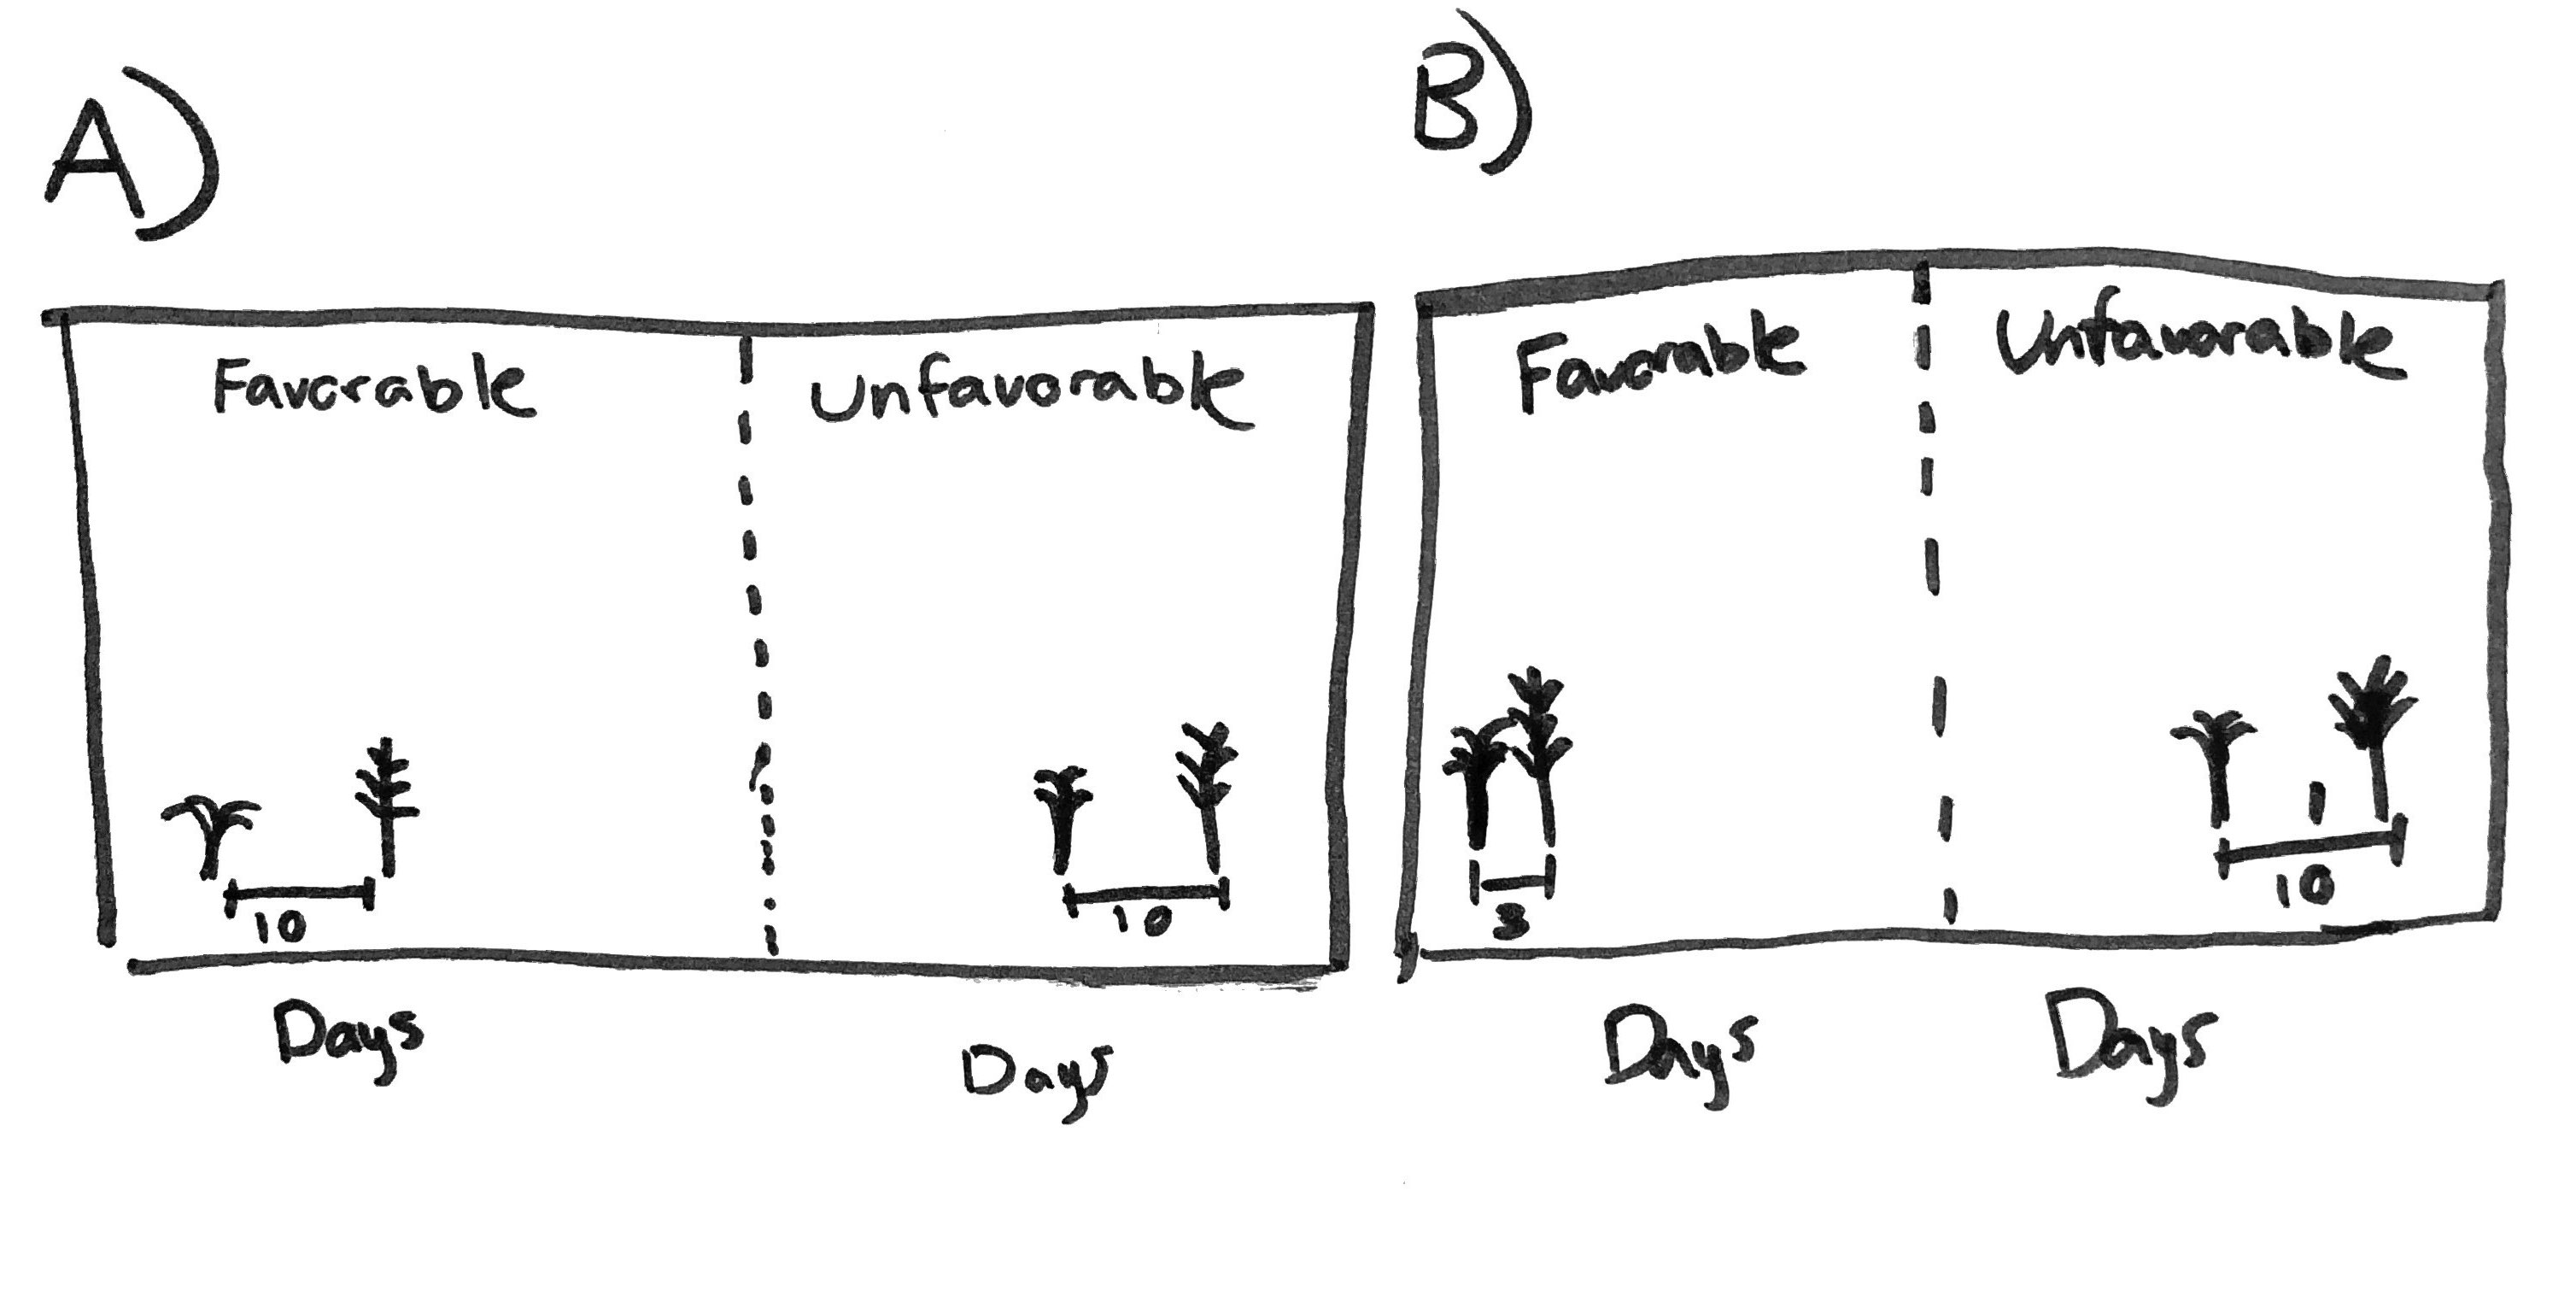
\includegraphics[width=\textwidth]{..//full_exp/concept_sketch.jpeg}
    \caption{ } 
    \label{fig:concept}
\end{figure}

\begin{figure}[h!]
    \centering
         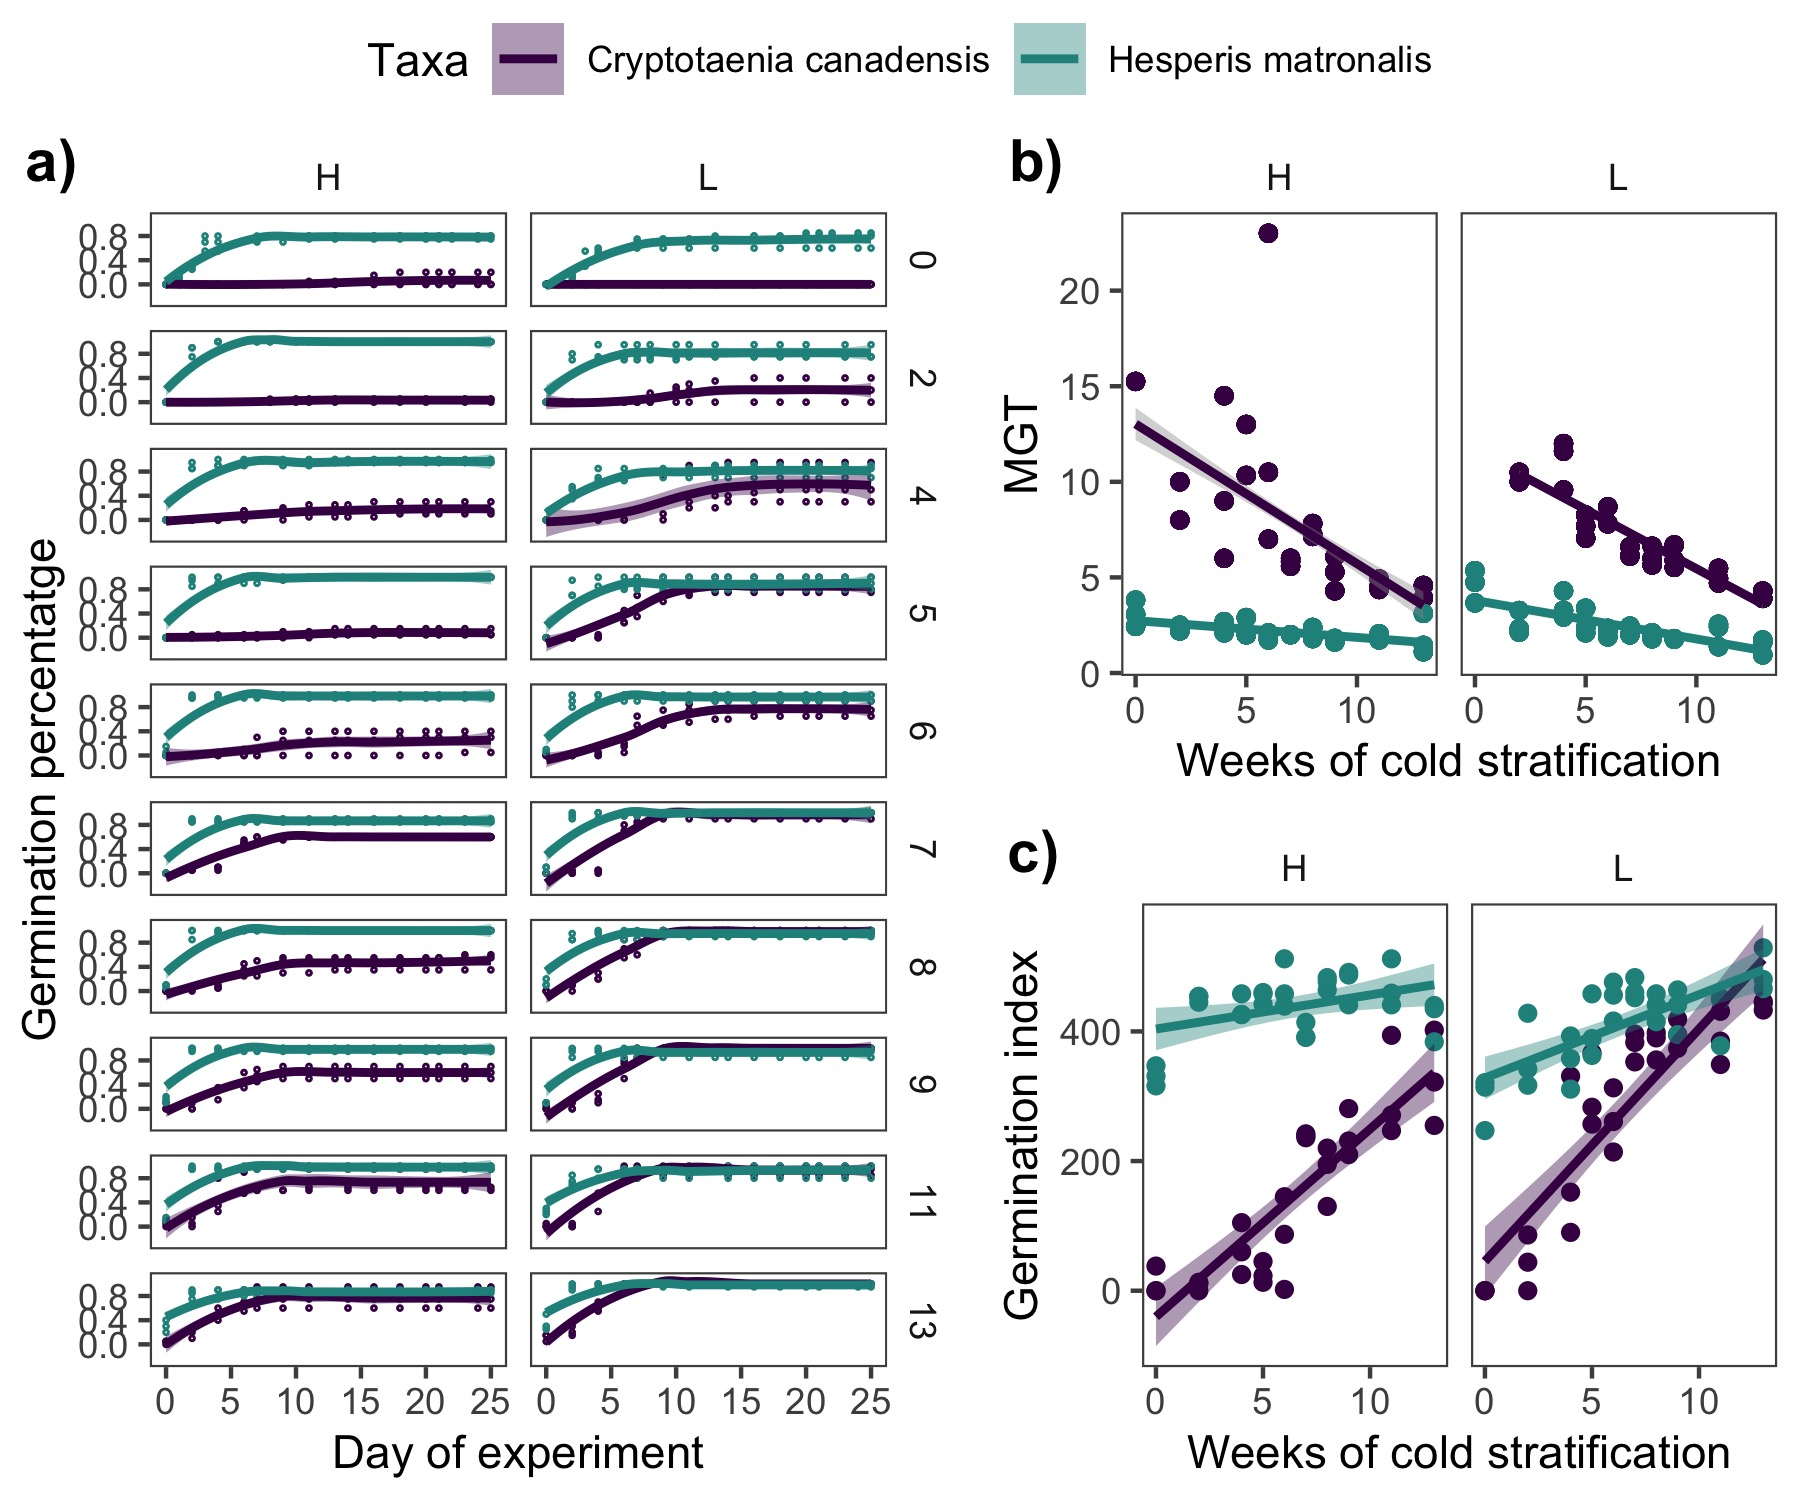
\includegraphics[width=\textwidth]{..//figure/crp_hesp1.jpeg}
    \caption{Germination behavior of \textit{H. matronalis} and \texit{C. canadensis} indicate that the rate of \texit{C. canadensis} approaches that of \textit{H. matronalis} under cool temperatures and high levels of stratification. } 
    \label{fig:aft}
\end{figure}

\begin{figure}[h!]
    \centering
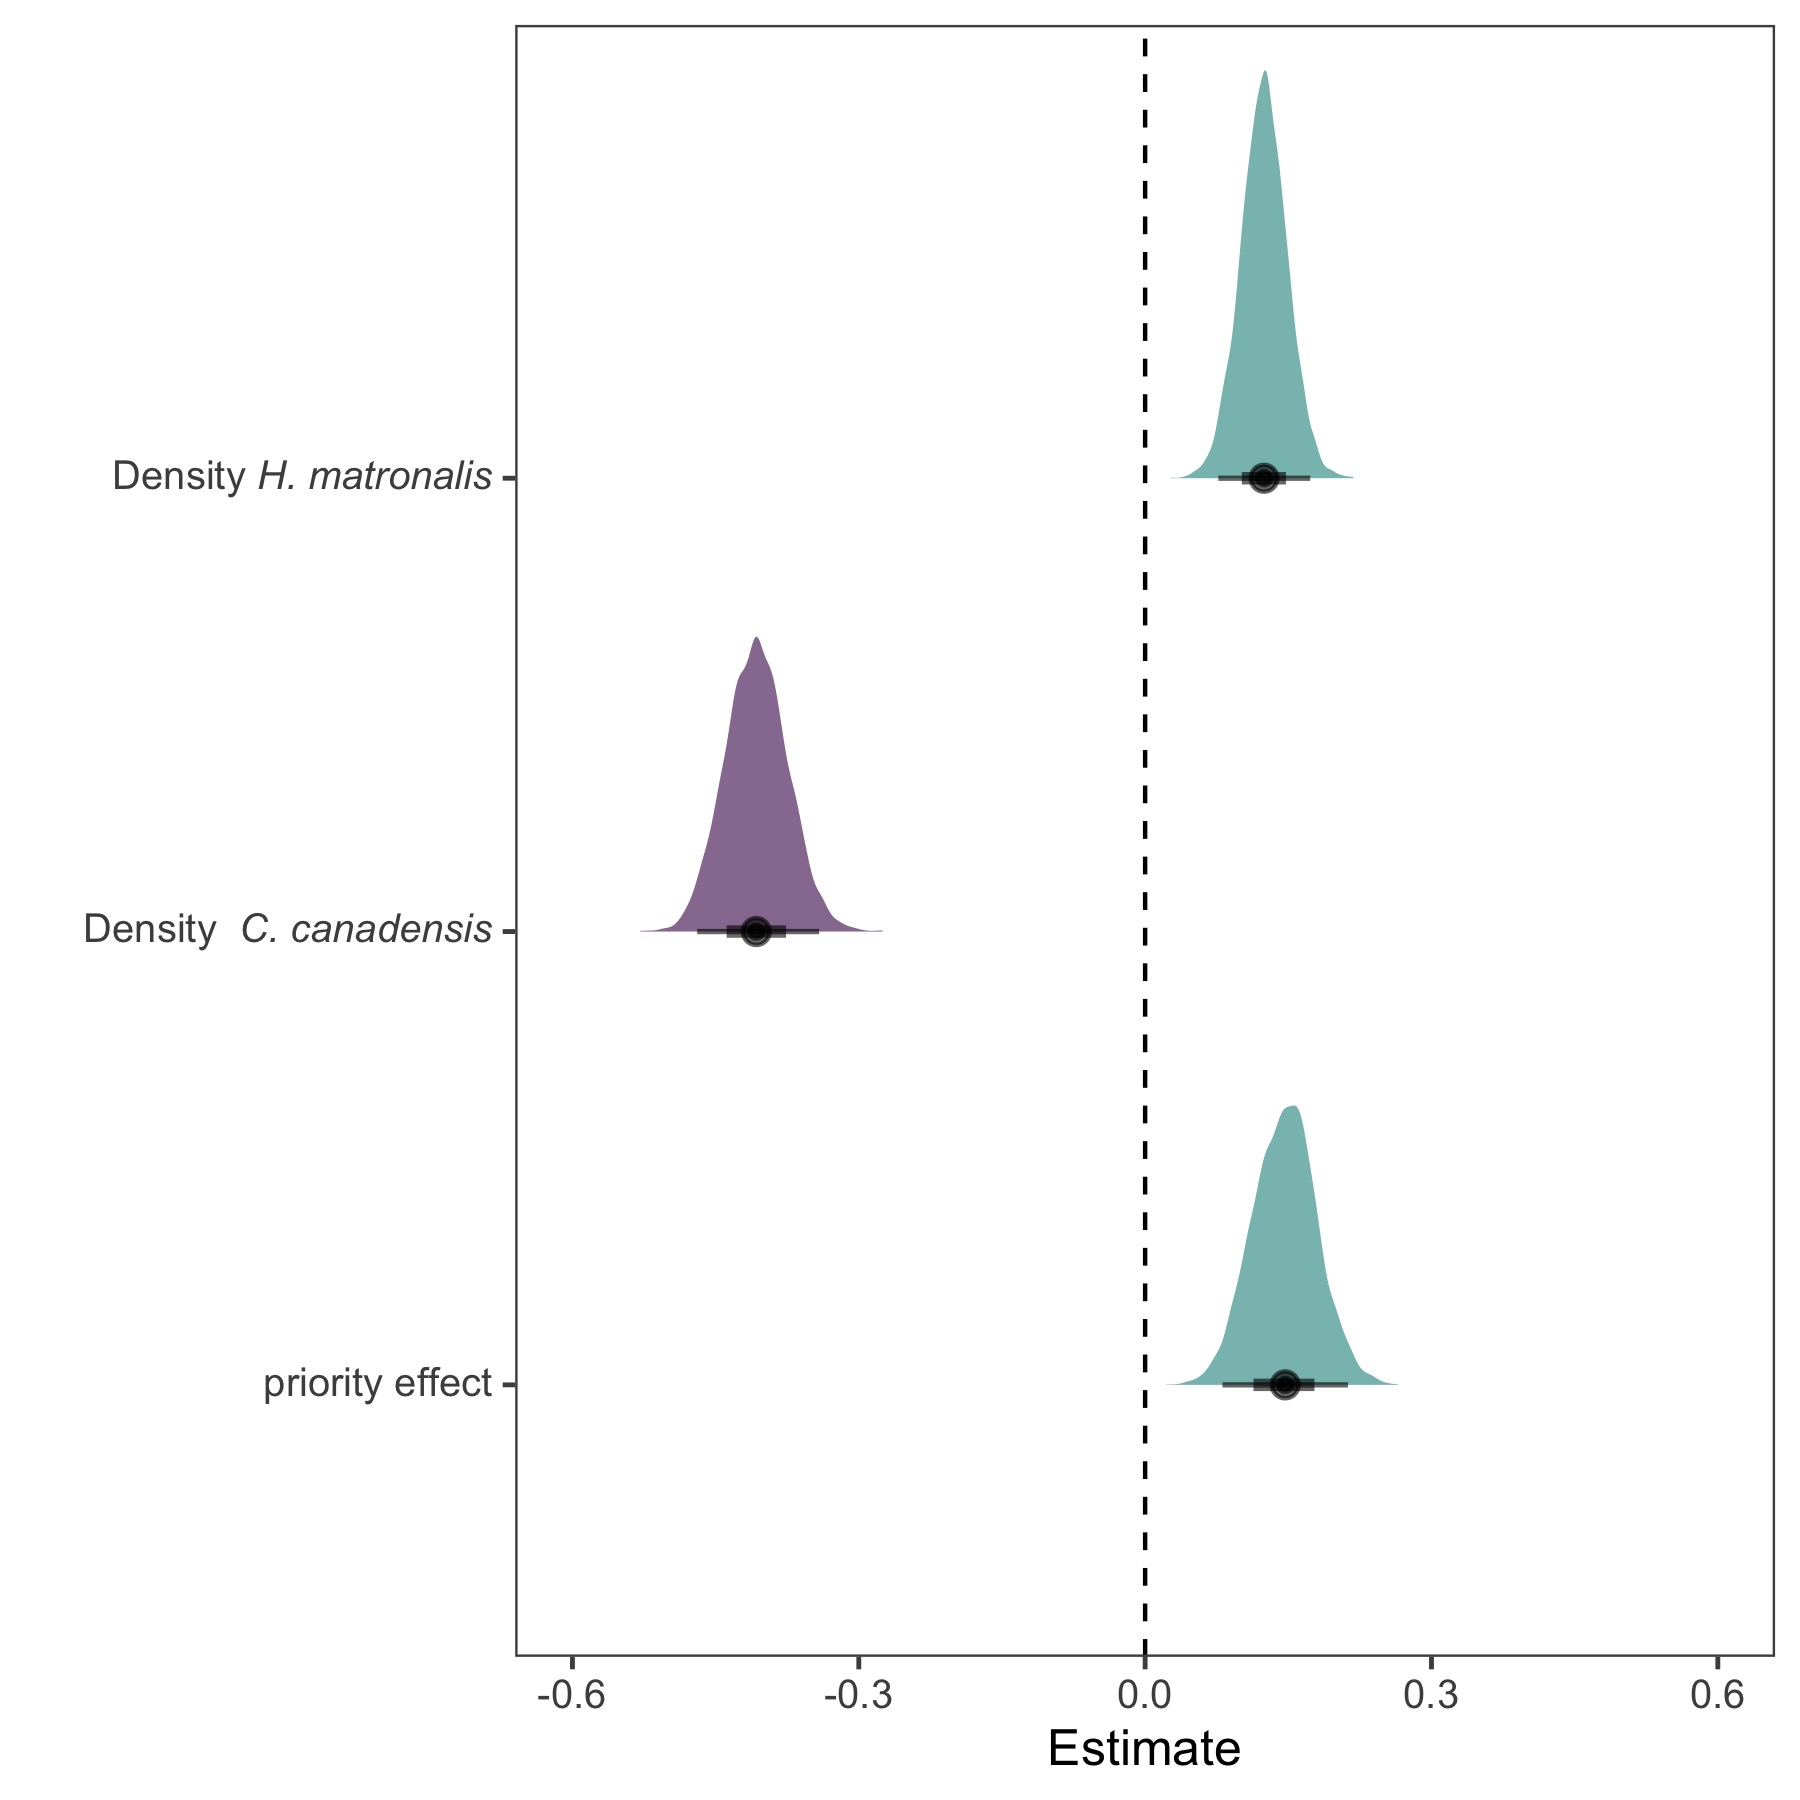
\includegraphics[width=\textwidth]{..//figure/mu_plots.jpeg}
    \caption{Estimated effects of density influence parameters and temporal priority effect on the relaive growth rate difference between \textit{H. matronalis} and \texit{C. canadensis}.  } 
    \label{fig:Cc}
\end{figure}

\begin{figure}[h!]
    \centering
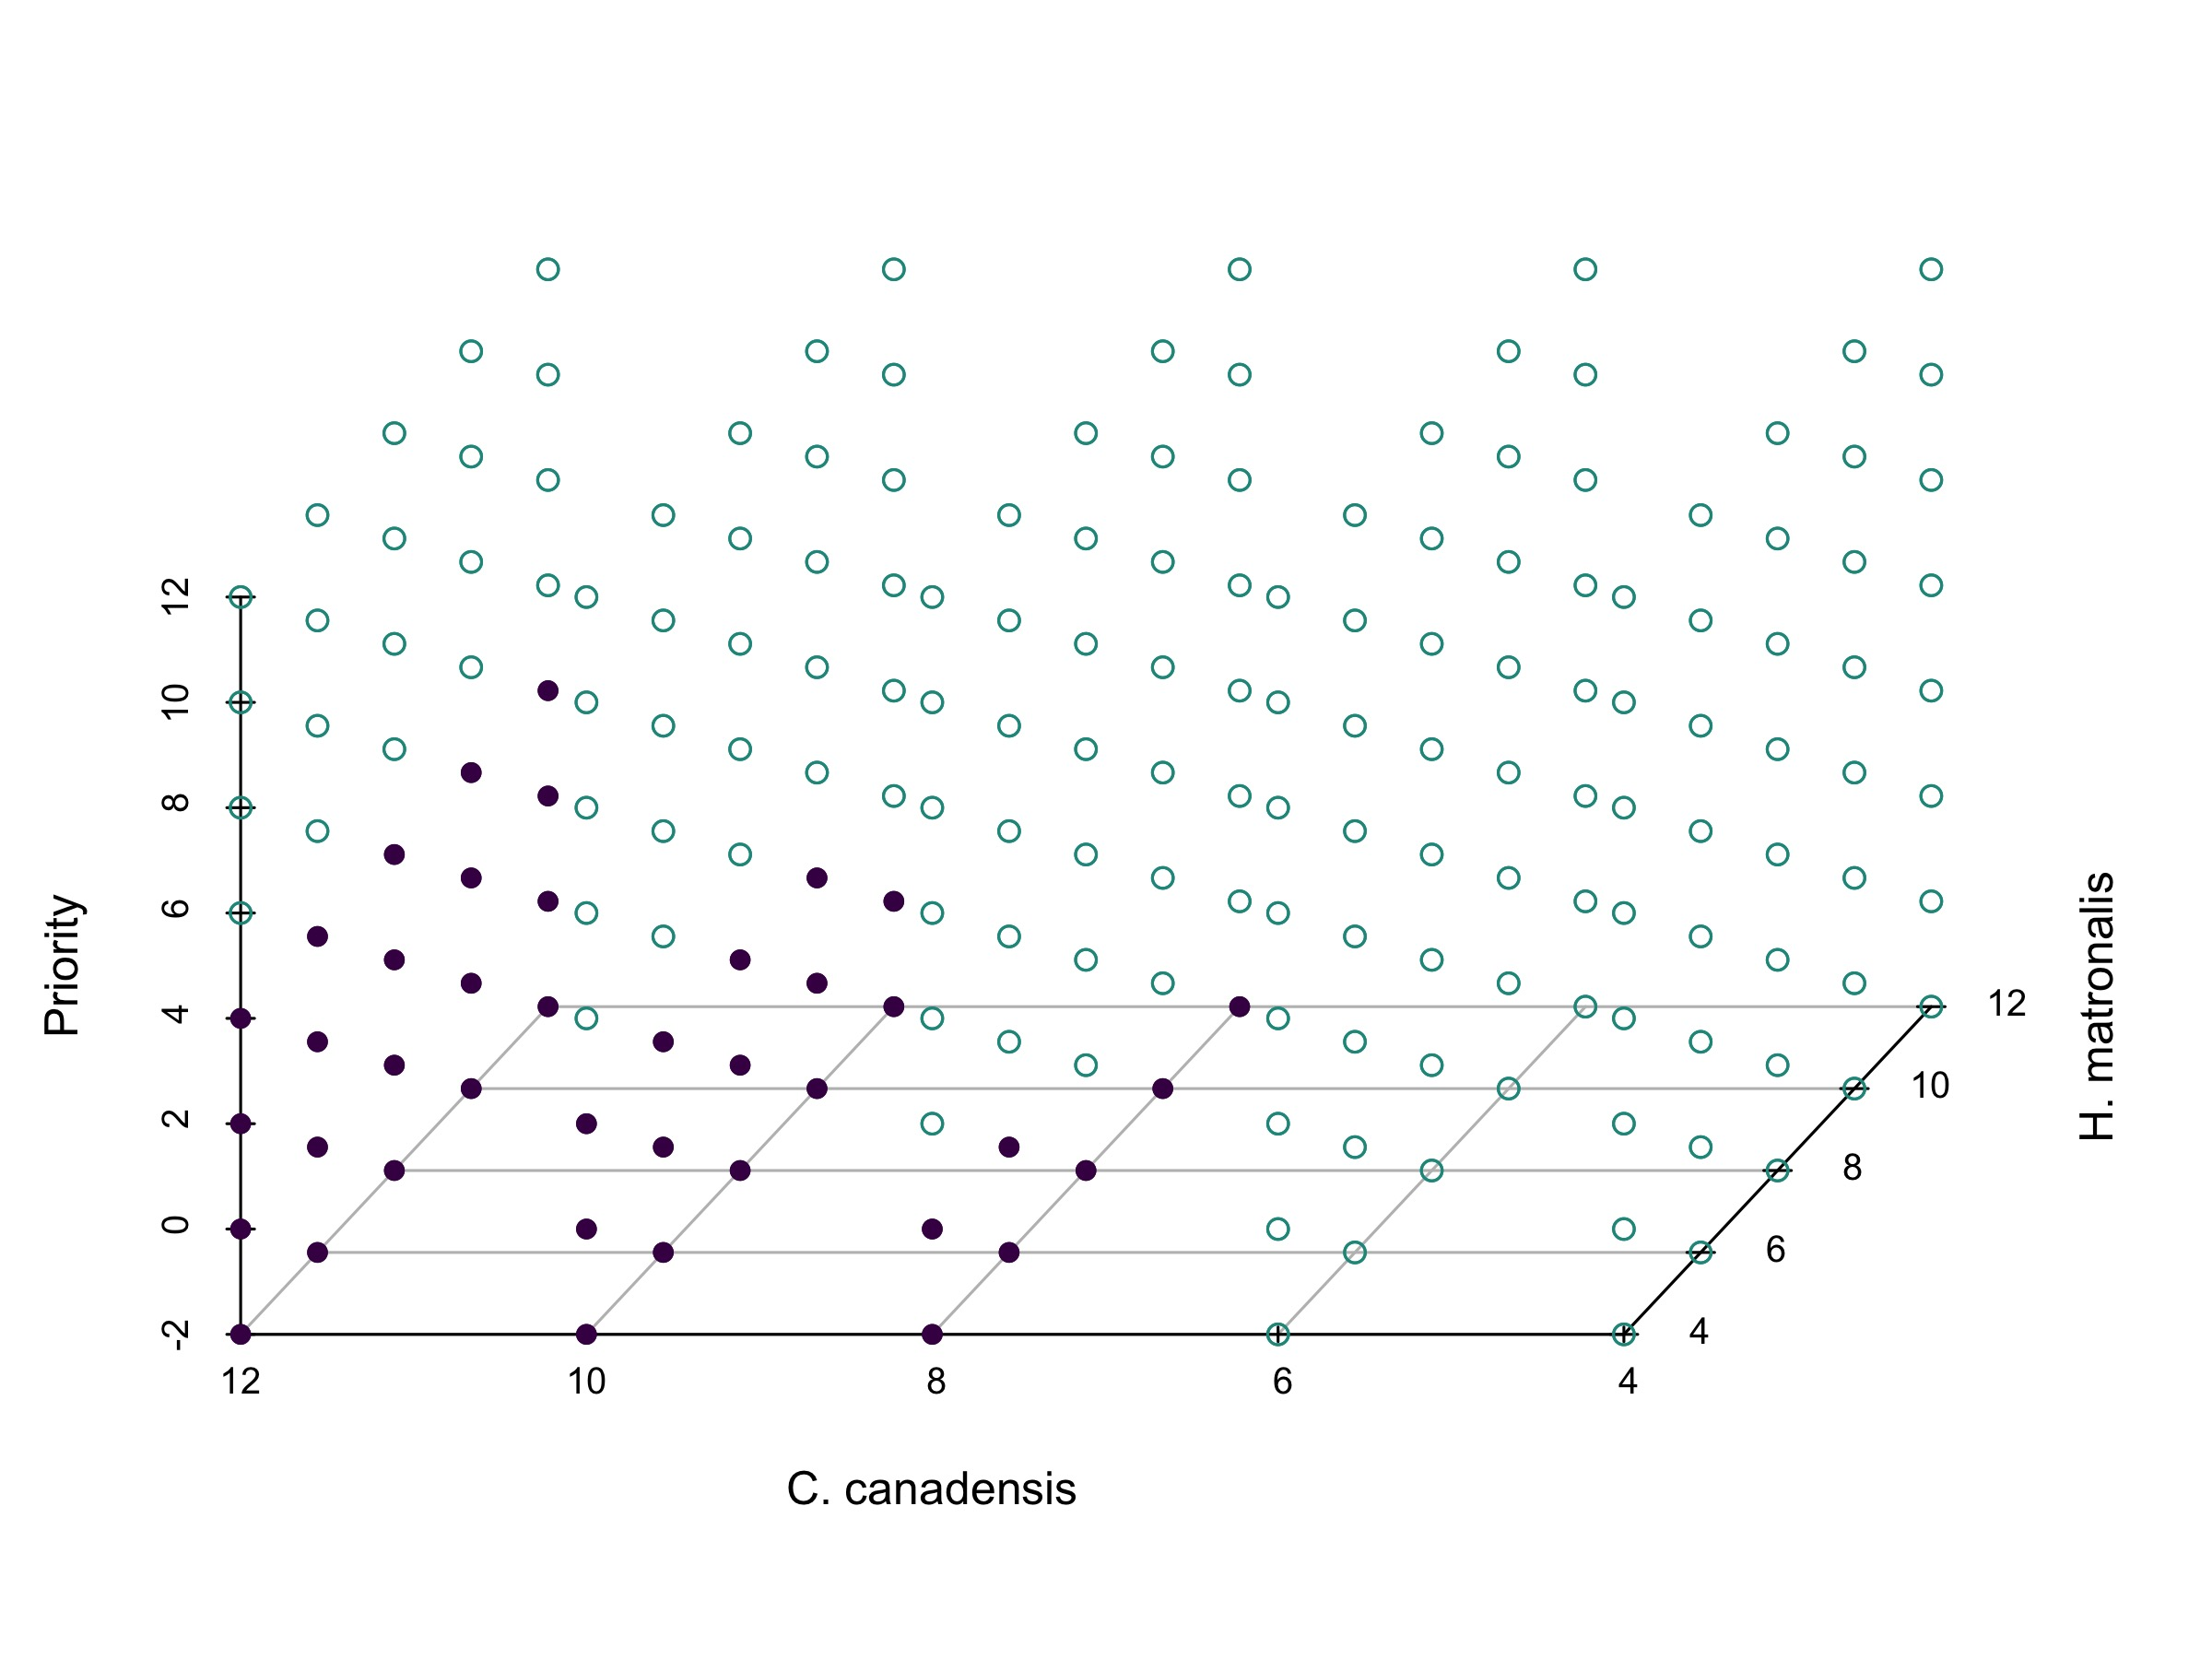
\includegraphics[width=\textwidth]{..//figure/threedpred.jpeg}
    \caption{Predicted outcome of competition under vary inter-specific densities and temporal priority. Purple is \texit{C. canadensis} and green \textit{H. matronalis}. Need to add legend here. } 
    \label{fig:Hm}
\end{figure}

\begin{figure}[h!]
    \centering
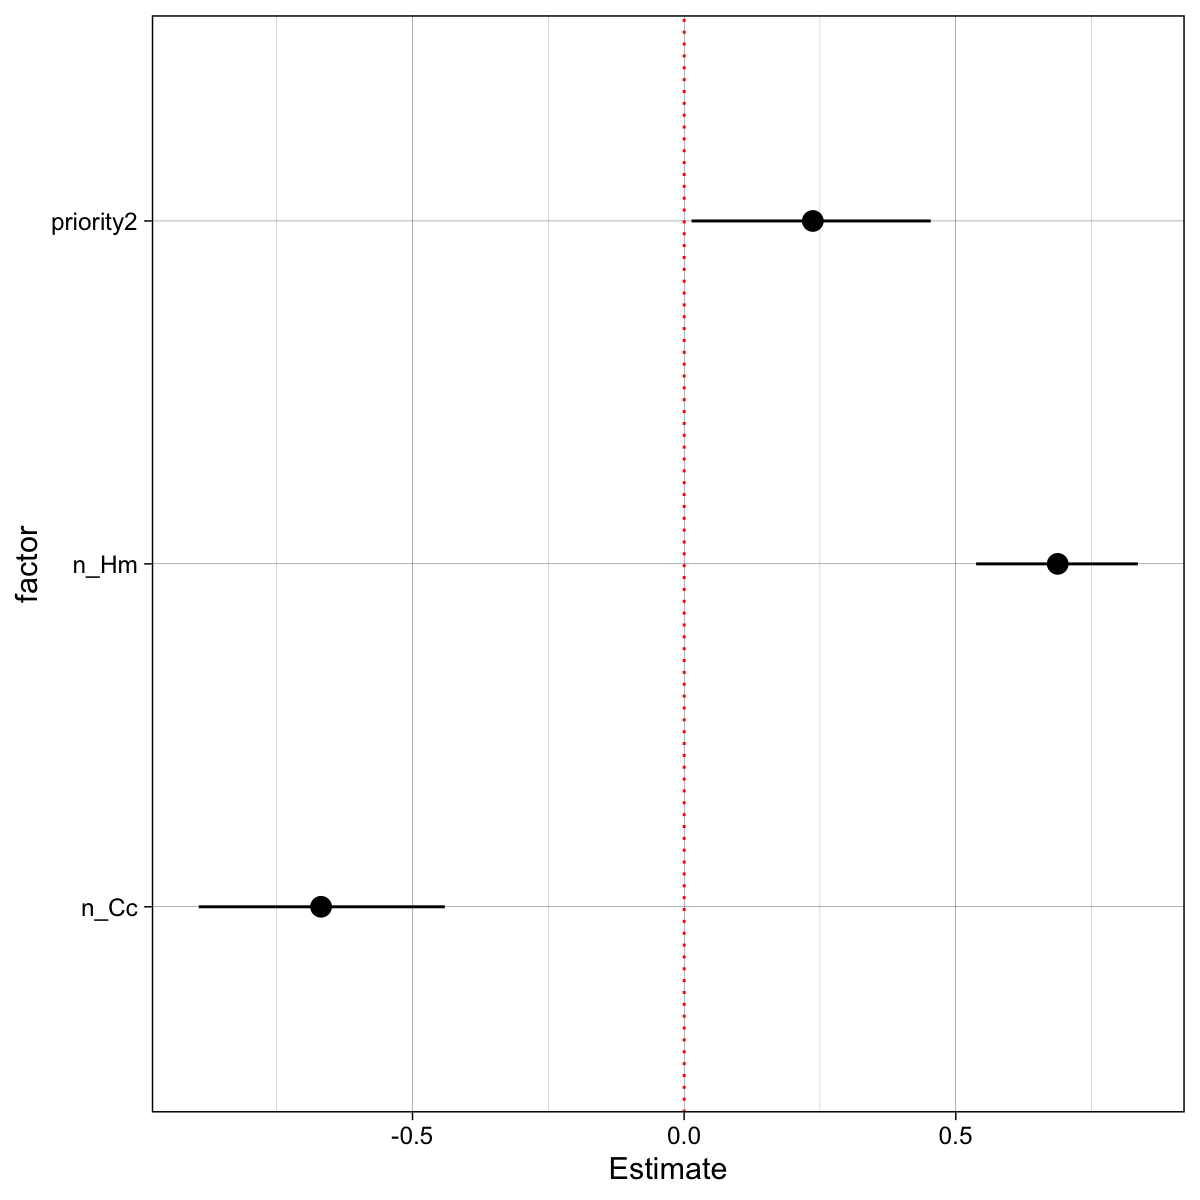
\includegraphics[width=\textwidth]{..//figure/RGRD_muplot.png}
    \caption{Very incomplete muplots based on equations from Connolly and Wayne 2005 (equations 2-4.) Currently doesn't factor in inital biomass (seed weight) or time interval. Betas supposively account for the ratio of intra to inter specific competition each species experiences. Positive values tip composition towards Hesperis and negative towards Cryptotaenia. } 
    \label{fig:Con}
\end{figure}

\end{document}
